% Compile with pdfLaTeX from the repository root or this directory.
% Content source: grade11/src/pages/term1/g11-t1-outline.html
\makeatletter
\def\input@path{{../../../preamble/}{book2026-2027/preamble/}}
\makeatother
\input{preamble.tex}

\geometry{letterpaper,margin=0.73in}
\linespread{1.06}
\setlength{\parskip}{4pt minus 3pt}
\setcounter{secnumdepth}{1}
\renewcommand{\thesection}{Step~\arabic{section}}
\hypersetup{pdftitle={Continuous Probability Distributions \& Risk},
  pdfsubject={Grade 11 Term 1 Outline},linkcolor=taskLinkDarkBlue}

\newcommand{\CriterionText}[2]{%
  {\small\textbf{\textcolor{taskLinkDarkBlue}{Criterion #1.}} #2\par}\smallskip}
\colorlet{eventFill}{black!24}

\begin{document}
\begin{center}
  {\LARGE\bfseries Continuous Probability Distributions \& Risk\par}
  \smallskip
  From density models and simulation to defensible financial risk conclusions.
  \par\medskip
  {\small Grade 11 \textperiodcentered{} Term 1 \textperiodcentered{} Outline\par}
\end{center}

\subsection*{From continuous models to measured risk}
Build, test, compare, and integrate probability models in one coherent investigation.

\section{Choose a distribution and find interval probabilities}

\subsection*{C1 --- Printing Orders}
\CriterionText{C1}{Characterises discrete and continuous random variables, identifies suitable distributions and supports, and interprets density and cumulative probability in context.}

\textbf{Count.} Orders arrive independently, one at a time, at a constant rate of 2 per hour. The number in one hour is \(\operatorname{Poisson}(2)\), with discrete support \(\{0,1,2,\ldots\}\).

\textbf{Measurement.} Poster completion time \(Y\) has continuous support \([10,30]\) minutes. Its density rises and falls along straight lines with a peak at 18, so use \(\operatorname{Tri}(10,30,18)\).

The density \(f(y)\) is a height in \(\mathrm{min}^{-1}\). The cumulative probability \(F(y)=P(Y\le y)\) is the area to the left. At the mode, \(F(18)=\frac{1}{2}\times8\times\frac{2}{20}=0.40\), so 40\% of poster orders finish within 18 minutes.

A general shape can fit several models. For example, a steadily decreasing density could be linear or curved.

\subsection*{C2 --- Market-stall Setup}
\CriterionText{C2}{Applies uniform and triangular models and constant or piecewise-linear densities to interval probabilities using geometric areas.}

Interval probability is area under the density. For a uniform model on \([a,b]\), multiply the interval length within the support by the rectangle's height \(\frac{1}{b-a}\). For a triangular model, set \(\frac{1}{2}\times(b-a)\times H=1\) to get peak height \(H=\frac{2}{b-a}\).

\begin{center}
  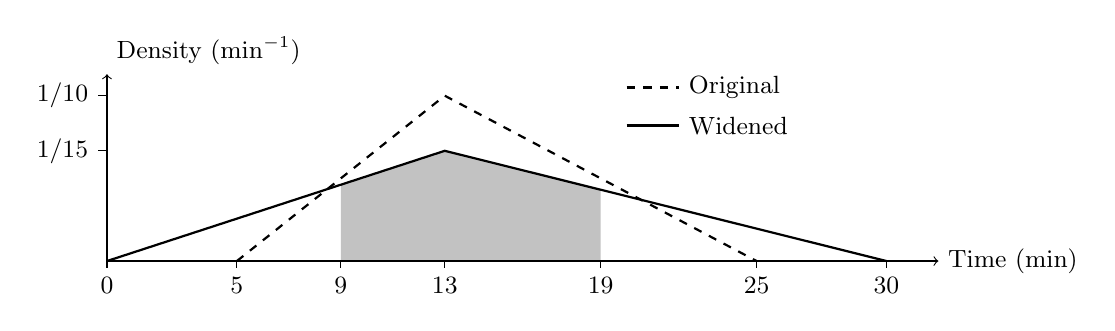
\begin{tikzpicture}[x=0.33cm,y=21cm,font=\small]
    \fill[eventFill] (9,0)--(9,{3/65})--(13,{1/15})--(19,{11/255})--(19,0)--cycle;
    \draw[thick] (0,0)--(13,{1/15})--(30,0);
    \draw[thick,dashed] (5,0)--(13,{1/10})--(25,0);
    \draw[->] (0,0)--(32,0) node[right]{Time (min)};
    \draw[->] (0,0)--(0,0.113) node[above right]{Density (\(\mathrm{min}^{-1}\))};
    \foreach \minute in {0,5,9,13,19,25,30}
      \draw (\minute,0)--++(0,-0.004) node[below]{\minute};
    \draw (0,{1/15})--++(-0.35,0) node[left]{\(1/15\)};
    \draw (0,{1/10})--++(-0.35,0) node[left]{\(1/10\)};
    \draw[thick,dashed] (20,0.105)--(22,0.105) node[right]{Original};
    \draw[thick] (20,0.082)--(22,0.082) node[right]{Widened};
  \end{tikzpicture}\par
  {\small Setup time is measured in minutes. The range widens from \([5,25]\) to \([0,30]\). The mode stays at 13.\par}
\end{center}

To find \(P(9\le S\le19)\), subtract the two tail triangles from 1. Get each tail height by scaling \(H\) along the straight branch.

\textbf{\([5,25]\).} \(H=\frac{2}{20}=\frac{1}{10}\). At 9 and 19, the heights are \(H\times\frac{4}{8}\) and \(H\times\frac{6}{12}\), both \(\frac{1}{20}\). The area is
\[
  1-\frac12\times4\times\frac1{20}-\frac12\times6\times\frac1{20}
  =\mathbf{0.7500}.
\]

\textbf{\([0,30]\).} \(H=\frac{2}{30}=\frac{1}{15}\). The heights become \(H\times\frac{9}{13}=\frac{3}{65}\) and \(H\times\frac{11}{17}=\frac{11}{255}\). The area is
\[
  1-\frac12\times9\times\frac3{65}-\frac12\times11\times\frac{11}{255}
  \approx\mathbf{0.5551}.
\]

\clearpage
\section{Find probabilities in cycles and waiting times}

\subsection*{C3 --- A Repeating Inspection Cycle}
\CriterionText{C3}{Uses circular geometry and arc proportions to calculate probabilities for uniform timing and directions around a circle.}

An alarm is equally likely to occur anywhere in a 60-minute cycle. For uniform timing or direction around a circle, divide the selected arc length by the full circumference, or use the equivalent fraction of time or angle.

\begin{center}
  \begin{minipage}{0.44\linewidth}
    \centering
    \begin{tikzpicture}[font=\small]
      \draw[gray,thick] (0,0) circle[radius=1.45];
      \draw[line width=2.2pt,-{Stealth}] (138:1.45)
        arc[start angle=138,end angle=24,radius=1.45];
      \fill (90:1.45) circle[radius=1.5pt] node[above=3pt]{\(60=0\)};
      \node[above left] at (138:1.45) {52};
      \node[right] at (24:1.45) {11};
      \node at (0,0) {60 min};
    \end{tikzpicture}
  \end{minipage}%
  \begin{minipage}{0.52\linewidth}
    The alarm window runs from minute 52 through the restart to minute 11.
    \[
      P=\frac{(60-52)+11}{60}=\frac{8+11}{60}=\frac{19}{60}\approx0.3167.
    \]
  \end{minipage}
\end{center}

\subsection*{C4 --- Exponential waits in both directions}
\CriterionText{C4}{Applies exponential models to constant-rate waiting times, infers event rates, and assesses model suitability.}

Use an exponential model for the wait to the next event in a constant-rate Poisson process. With time \(t\) in minutes and rate \(\lambda\) per minute, \(P(T>t)=e^{-\lambda t}\).

\textbf{Charging-space Availability --- Rate to probability.} At 12 openings per hour, \(\lambda=\frac{12}{60}=\frac{1}{5}\) per minute. For a wait under 3 minutes or over 8 minutes, add the disjoint tails.
\[
  P(T<3\text{ or }T>8)=(1-e^{-3/5})+e^{-8/5}\approx0.6531.
\]

\textbf{Electronic Receipt Rates --- Probability to rate.} In the morning, \(P(T>10)=0.40\). Set \(e^{-10\lambda}=0.40\) and take natural logs. Then \(\lambda=-\frac{\ln(0.40)}{10}\) receipts per minute, or \(60\lambda\approx\mathbf{5.498}\) \textbf{receipts per hour}.

\clearpage
\section{Compare theoretical and sample results}

\subsection*{C5 --- Two Labelling Stations}
\CriterionText{C5}{Calculates and interprets the mean, variance, and standard deviation of continuous distributions using standard formulas.}

Both labelling times are on \([3,15]\) minutes. Station A has a triangular density rising to a mode of 15. Station B has a uniform density.

\begin{center}
  {\small Theoretical mean and spread at the two stations\par}\smallskip
  \begin{tabular}{@{}lcc@{}}
    \toprule
    \textbf{Statistic} & \textbf{Station A} & \textbf{Station B}\\
    \midrule
    Mean (min) & \(\dfrac{3+2\times15}{3}=11\) & \(\dfrac{3+15}{2}=9\)\\[8pt]
    Variance (\(\mathrm{min}^2\)) & \(\dfrac{(15-3)^2}{18}=8\) & \(\dfrac{(15-3)^2}{12}=12\)\\[8pt]
    SD (min) & \(\sqrt{8}\approx2.828\) & \(\sqrt{12}\approx3.464\)\\
    \bottomrule
  \end{tabular}
\end{center}

Station A takes longer on average and has a smaller standard deviation.

\subsection*{C6 --- File Transfers}
\CriterionText{C6}{Estimates interval probabilities using sample relative frequencies and compares them with theoretical probabilities.}

For \(4\le X<12\) seconds, add the counts from \([4,8)\) and \([8,12)\) to get \(9+5=14\). The four classes have \(3+9+5+3=20\) observations, giving an empirical probability of \(\frac{14}{20}=\mathbf{0.70}\).

Against the model probability 0.75, the absolute error is \(\lvert0.70-0.75\rvert=\mathbf{0.05}\). The percentage error is \(\frac{0.05}{0.75}\times100\%\approx\mathbf{6.67\%}\). Counts can come from raw data, grouped frequencies, or a histogram.

\subsection*{C7 --- Courier Routes}
\CriterionText{C7}{Calculates sample means, variances, and standard deviations for different sample sizes and data representations and compares them with theory.}

\begin{center}
  {\small Represent each route-time class by its midpoint.\par}\smallskip
  \begin{tabular}{@{}lcc@{}}
    \toprule
    \textbf{Class (min)} & \textbf{Midpoint} & \textbf{Count}\\
    \midrule
    \([8,12)\) & 10 & 2\\
    \([12,16)\) & 14 & 3\\
    \([16,20)\) & 18 & 1\\
    \bottomrule
  \end{tabular}
\end{center}

With \(n=6\), the midpoint estimate of the sample mean is
\[
  \bar{x}=\frac{2\times10+3\times14+18}{6}=\frac{40}{3}\approx\mathbf{13.333}\,\mathrm{min}.
\]
Weight each squared deviation by its count. The sum is
\[
  2(10-\bar{x})^2+3(14-\bar{x})^2+(18-\bar{x})^2=\frac{136}{3}\,\mathrm{min}^2.
\]
Divide by \(n-1=5\) to estimate \(s^2=\frac{136}{15}\approx\mathbf{9.067}\,\mathrm{min}^2\). Take its square root for \(s\approx\mathbf{3.011}\,\mathrm{min}\).

Using the unrounded estimates, the mean differs from 14 min by 0.667 min (4.76\%) and the variance differs from 12 \(\mathrm{min}^2\) by 2.933 \(\mathrm{min}^2\) (24.44\%). In each case, divide the absolute error by the theoretical value and multiply by 100\%.

\clearpage
\section{Read Student's \texorpdfstring{\(t\)}{t} tables and compare models}

\subsection*{C8 --- From cutoffs to areas and back}
\CriterionText{C8}{Uses Student's \(t\)-distribution tables, degrees of freedom, and one-tailed or two-tailed areas to determine critical values, central probabilities, and tail probabilities or probability ranges.}

For the supplied model \(X=m+aT\), use \(\mathrm{df}=n-1\). The \(t\) table pairs a positive critical value with its right-tail area. By symmetry, the negative critical value has the same area to its left.

\textbf{Direct --- Retail Revenue Alerts.} For \(n=7\), \(m=2\) and \(a=4\), standardise with \(c=\frac{x-m}{a}\). The cutoffs give \(\frac{-5.772-2}{4}=-1.943\) and \(\frac{7.76-2}{4}=1.440\). Row 6 gives tail areas 0.05 and 0.10.

\begin{center}
  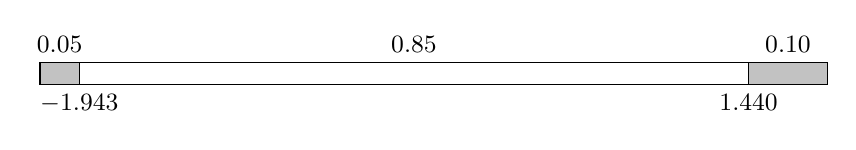
\begin{tikzpicture}[x=10cm,font=\small]
    \fill[eventFill] (0,0) rectangle (0.05,0.28);
    \fill[eventFill] (0.90,0) rectangle (1,0.28);
    \draw (0,0) rectangle (1,0.28);
    \draw (0.05,0.28)--(0.05,0) node[below]{\(-1.943\)};
    \draw (0.90,0.28)--(0.90,0) node[below]{\(1.440\)};
    \node[above] at (0.025,0.28) {0.05};
    \node[above] at (0.475,0.28) {0.85};
    \node[above] at (0.95,0.28) {0.10};
  \end{tikzpicture}\par
  {\small Add the two alert tails. The alert probability is approximately \(0.05+0.10=0.15\).\par}
\end{center}

\textbf{Inverse --- Dispatch Time Alerts.} With \(n=16\), use row 15. The 0.01 lower tail gives \(c_L=-2.602\) by symmetry, and the 0.10 upper tail gives \(c_U=1.341\). Back-transform with \(x=m+ac\).
\[
  L=-2+6(-2.602)\approx-17.61\,\mathrm{min},
  \qquad U=-2+6(1.341)\approx6.05\,\mathrm{min}.
\]

\subsection*{C9 --- Sales Revenue Shortfalls}
\CriterionText{C9}{Calculates and compares critical values and probability areas from the standard normal and Student's \(t\)-distributions, selecting and justifying the appropriate distribution according to whether the population standard deviation is known or estimated from the sample.}

Compare \(P(X<-11.165)\) for \(X_T=-2+5T\) and \(X_N=-2+5Z\), with \(T\) from the \(t\) model (\(\mathrm{df}=9\)) and \(Z\) standard normal. Both use the supplied location \(-2\) and take the stated approximate standard deviation of 5 as the common scale, in thousands of dollars. The resulting standard deviations are 5 for \(X_N\) and \(5\sqrt{9/7}\) for \(X_T\).

\textbf{Table-based comparison of the same shortfall under both models.}
Standardise once to get \(\frac{-11.165+2}{5}=-1.833\). Row 9 of the \(t\) table gives a left tail of \textbf{0.0500} by symmetry. For normal, round to \(z=-1.83\) and use \(1-\Phi(1.83)\), which gives \(1-0.9664=\mathbf{0.0336}\).

The absolute difference is \(\lvert0.0500-0.0336\rvert=\mathbf{0.0164}\). Divide by each model's probability to get the relative differences.
\[
  \frac{0.0164}{0.0500}\times100\%=32.80\%\quad\text{relative to }t,
  \qquad
  \frac{0.0164}{0.0336}\times100\%\approx48.81\%\quad\text{relative to normal}.
\]

For inverse comparisons, look up each model's critical values at the same target areas, then back-transform to the original units before calculating differences. For an interval, compare lower endpoints and upper endpoints separately.

\clearpage
\section{Integrate the methods in a risk investigation}
\CriterionText{C10}{Integrates continuous probability modelling, simulation, sampling analysis, and portfolio-risk measures to investigate an economic or financial question, justifying the selected methods and communicating results, assumptions, limitations, and evidence-based conclusions.}

Ask whether a 60\% bond / 40\% equity portfolio meets a return target without excessive volatility. Select continuous return models, simulate outcomes, compare sample evidence with theoretical mean and variance, and use justified \(z\)/\(t\) reasoning. Report assumptions, limitations, and a recommendation supported by both probability and portfolio risk.

\subsection*{C10 --- From a financial question to an evidence-based recommendation}

\begin{center}
  \begin{tikzpicture}[
    node distance=0.55cm,
    stage/.style={draw,rounded corners=2pt,align=center,font=\small,
      text width=1.8cm,minimum height=1.05cm},
    >={Stealth}]
    \node[stage] (question) {Question\\\& data};
    \node[stage,right=of question] (model) {Select\\model};
    \node[stage,right=of model] (simulation) {Simulate\\\& sample};
    \node[stage,right=of simulation] (risk) {Measure\\risk};
    \node[stage,right=of risk] (conclusion) {Conclude\\\& qualify};
    \draw[->] (question)--(model);
    \draw[->] (model)--(simulation);
    \draw[->] (simulation)--(risk);
    \draw[->] (risk)--(conclusion);
  \end{tikzpicture}
\end{center}

\[
  \sigma_p^2=w_B^2\sigma_B^2+w_E^2\sigma_E^2
    +2w_Bw_E\rho_{BE}\sigma_B\sigma_E.
\]

\begin{center}
  \begin{tabular}{@{}lccc@{}}
    \toprule
    \textbf{Input} & \textbf{Bond \(B\)} & \textbf{Equity \(E\)} & \textbf{Portfolio}\\
    \midrule
    Weight & 0.60 & 0.40 & 1.00\\
    Expected return & 4\% & 10\% & \textbf{6.4\%}\\
    Volatility & 5\% & 15\% & \textbf{7.22\%}\\
    \bottomrule
  \end{tabular}
\end{center}

Here \(\rho_{BE}=0.20\) is return correlation, \(w\) is asset weight, and \(\sigma\) is return standard deviation. Portfolio variance is 0.00522, so \(\sigma_p=\sqrt{0.00522}\approx0.0722\). Conclusions remain conditional on stable parameters and a representative sample.

\end{document}
